\documentclass[11pt]{beamer}

\usetheme{classic}
\usefonttheme{structurebold}

%%%%PACKAGES%%%%%%%%%%%%%%%%
\usepackage{times}
\usepackage[spanish,english]{babel}
\usepackage{amsmath,amssymb}
\usepackage[latin1]{inputenc}
\usepackage{bm}


\setbeamercovered{dynamic}


%NEWCOMMANDS%%%%%%%%%%%%%%%%%%%%
\def\'#1{\if#1i{\accent19\i}\else{\accent19#1}\fi} % -> \'{\i}

%%%%%%%%%%%%%%%%%%%%%%%%%%%%%%%%

\AtBeginSection[]{\frame{\frametitle{Outline}\tableofcontents[current]}}


%TITLE_PAGE%%%%%%%%%%%%%%%%%%%
\title{\textcolor{darkgreen}{Topics}}
\institute{\large \textcolor{darkblue}{Centro de Investigaciones en \'Optica (CIO)}}
\date{\alert{}}


%BEGIN >>>>>>>>>>>>>>>>>>>>>>>>>
\begin{document}

%%%%%%%%%%%%%%%%%%%%%%%%%
\section{Capas y nanotubos}
\begin{frame} \frametitle{Nanotubos de silicio}

\begin{minipage}{.44\textwidth}
\begin{itemize}
\item Estructura electr\'onica y 
 respuesta \'optica lineal de capas y nanotubos 
 de silicio.
\end{itemize}
\begin{center}
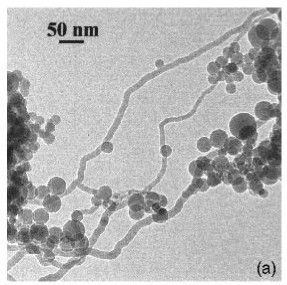
\includegraphics[scale=.45]{pictures/TEM-SiNT-a.jpg}
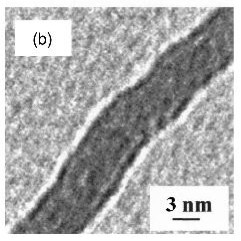
\includegraphics[scale=.45]{pictures/TEM-SiNT-b.jpg}\\
{\tiny {\sc Imagenes TEM de nanotubos de Silicio [Crescenzi, APL
    (2005)]}}\\
\vfill
\end{center}
\end{minipage}
\begin{minipage}{.55\textwidth}
\begin{center}
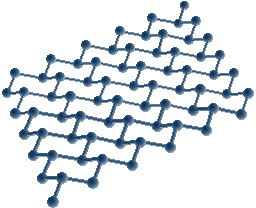
\includegraphics[scale=.3]{pictures/Silicene.jpg}
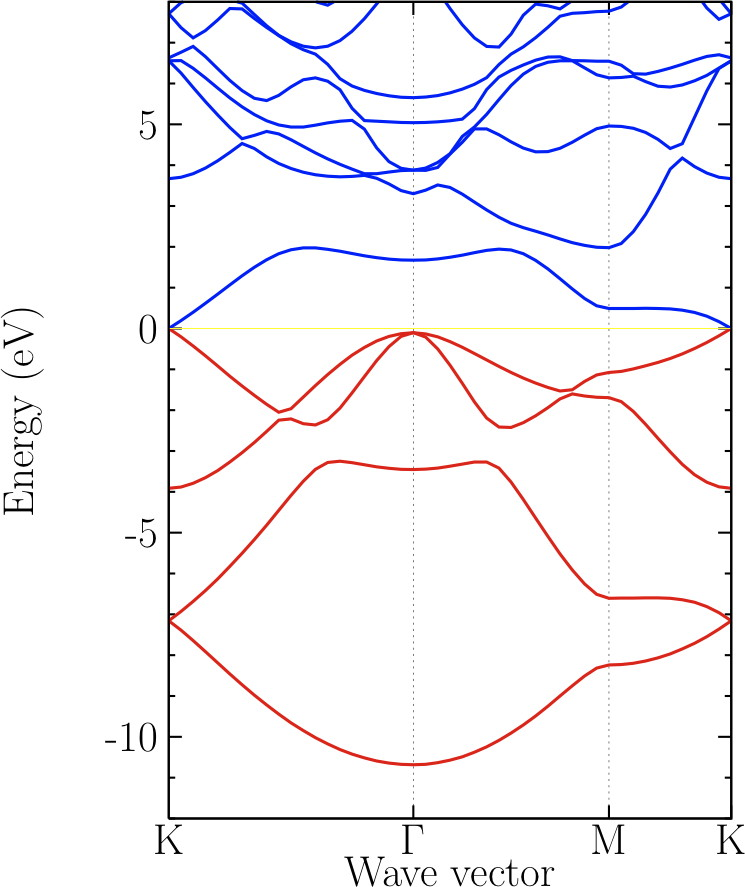
\includegraphics[scale=.22]{pictures/si-glayer-energies.jpg} \\
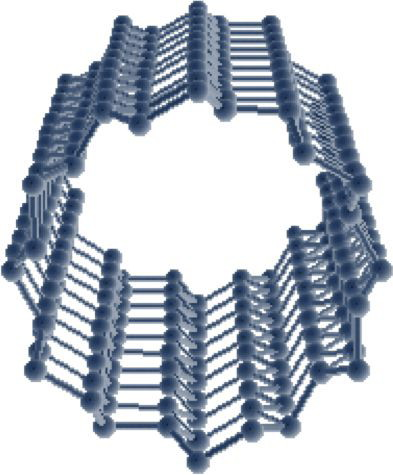
\includegraphics[scale=.3]{pictures/si66-frontView.jpg} \hspace{7mm}
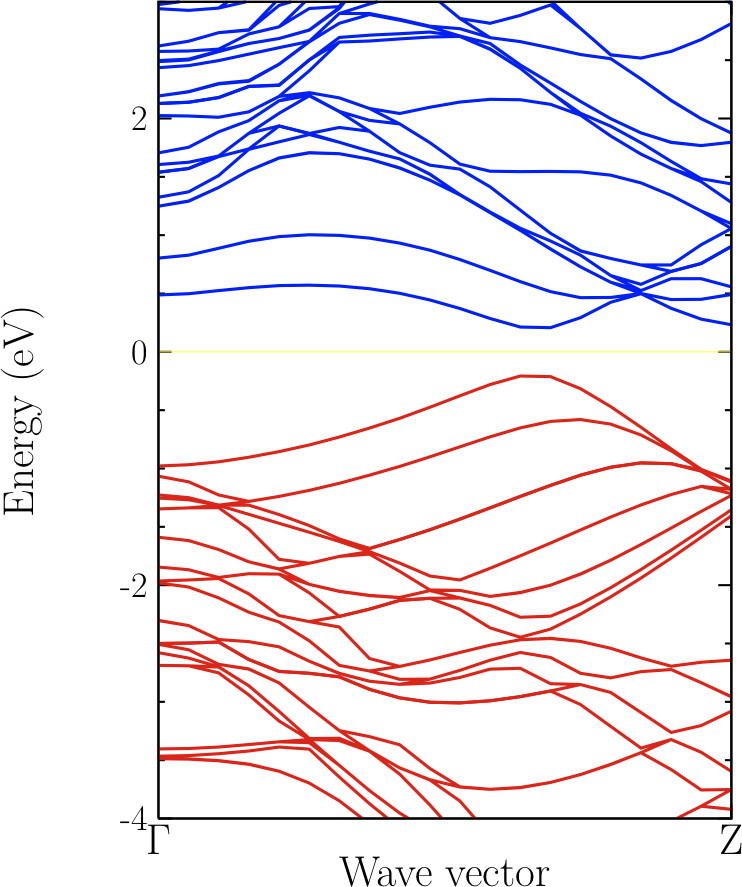
\includegraphics[scale=.22]{pictures/g-si66-energies.jpg} \\
\end{center}
\end{minipage}

\end{frame}
%%%%


%%%%%%%%%%%%%%%%%%%%%%%%%
\begin{frame} \frametitle{Nanotubos de silicio}

\begin{minipage}{.54\textwidth}
\begin{itemize}
\item Estudio de la respuesta \'optica lineal y 
   grado de polarizaci\'on de esp\'in en capas y nanotubos
  de silicio como funci\'on  de la cobertura de hidr\'ogeno.
\end{itemize}
\begin{center}
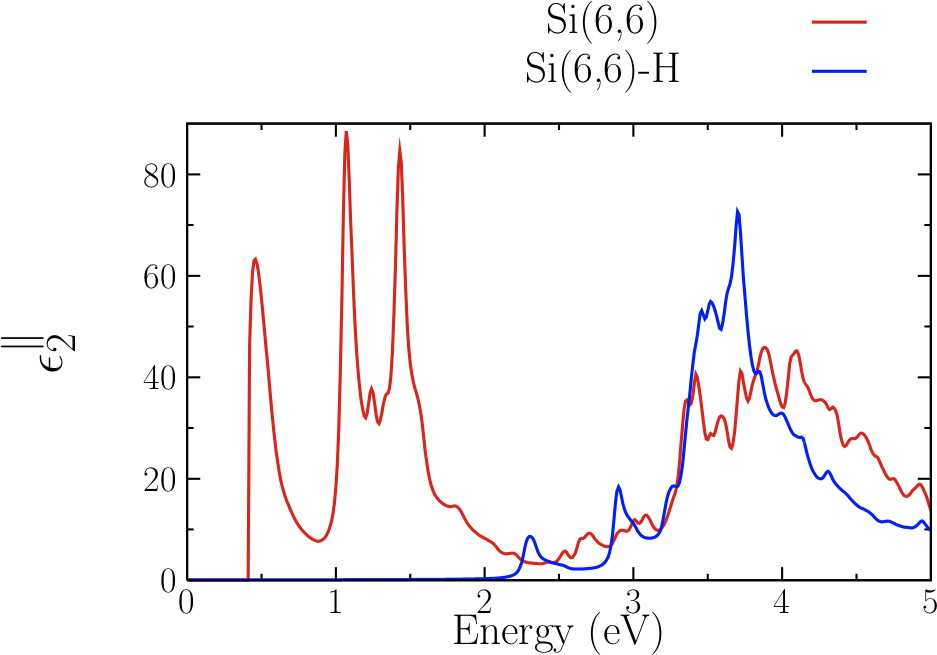
\includegraphics[scale=.4]{pictures/si66-eps-parallel.jpg}
\end{center}
\end{minipage}
\begin{minipage}{.44\textwidth}
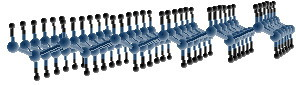
\includegraphics[scale=.5]{pictures/silicane.jpg}
\vfill
\centerline{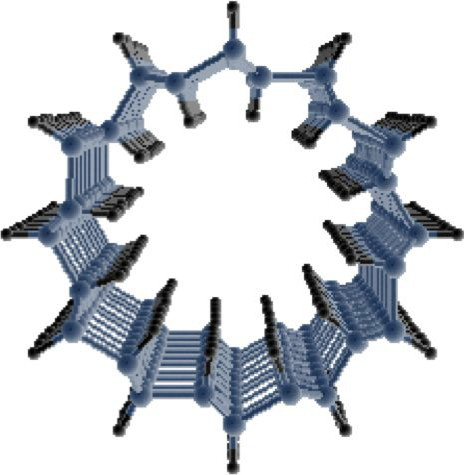
\includegraphics[scale=.4]{pictures/si66-H-frontView.jpg}}
\vfill
\end{minipage}
\vfill

\end{frame}
%%%%

\end{document}
% <<<<<<<<<<<<

